\subsection{Simulation with simulink}

A simulation was done using Simulink to compare the tracking behaviour between
simulation and experiment. Unfortunately  the  time  in the laboratory was not
enough  to finish the exercise. So we didn't have  the  time  to  analyse  the
tracking behaviour of the electrical motor  in  the  laboratory.  However,  in
Simulink  the  tracking  behaviour was analysed and it can be seen  in  figure
\ref{fig:tracking}. The best value for  the  $PT_{1}$-element we determined to
be $5.962$, so our $PT_{1}$-element is of the form:

\begin{equation}
    G(s) = \frac{1}{5.962s+1}
\end{equation}

For  the   dead   time   element   we  took  the  value  $0.1655$.  In  figure
\ref{fig:simulink} there are 5  different  Block  diagram. the first 3 diagram
represent  the  simulation  model  of  the  plant. The last two Block  diagram
represent an implemented PID controller with and without a tracking behaviour.

The best PID controller we obtained  during  the  experiment  have  the values
(Proportional $P$, Integral $I$ and Derivative $D$) :

\begin{align*}
    P &= 0.330 \\
    I &= 0.660 \\
    D &= 0.330
\end{align*}

\begin{figure}[t]
    \centering
    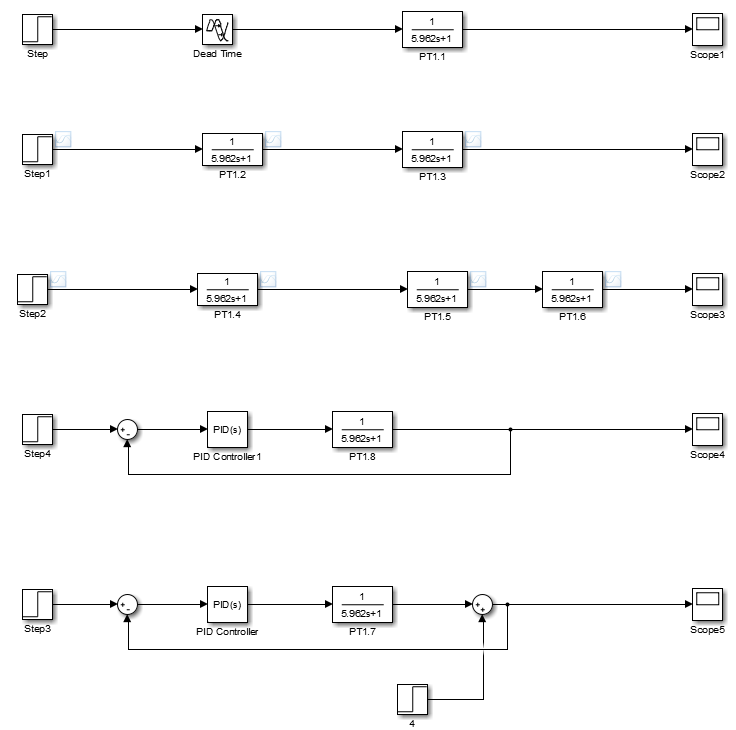
\includegraphics[width=\imagewidth]{images/simulink.png}
    \caption{Block diagram of the Simulink simulation}
    \label{fig:simulink}
\end{figure}

The smallest tracking behaviour we obtained with the values:

\begin{align*}
    P &= 0.330 \\
    I &= 0.660 \\
    D &= 0.330
\end{align*}

which  are  the  same  as  for  the  normal   PID   controller.   In   picture
\ref{fig:tracking}  one  can  see  that the tracking behaviour have a change of
$180$  degree.  That means that the electrical  motor  change  his  direction.

\begin{figure}[t]
    \centering
    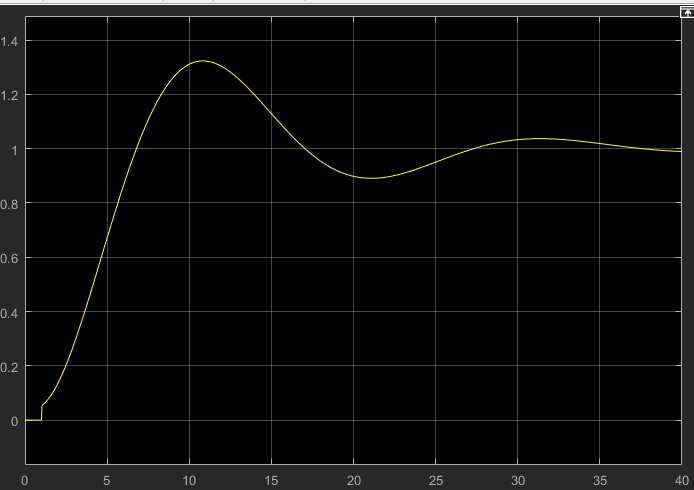
\includegraphics[width=\imagewidth]{images/slope.png}
    \caption{The system without tracking.}
    \label{fig:WithoutTracking}
\end{figure}

\begin{figure}[t]
    \centering
    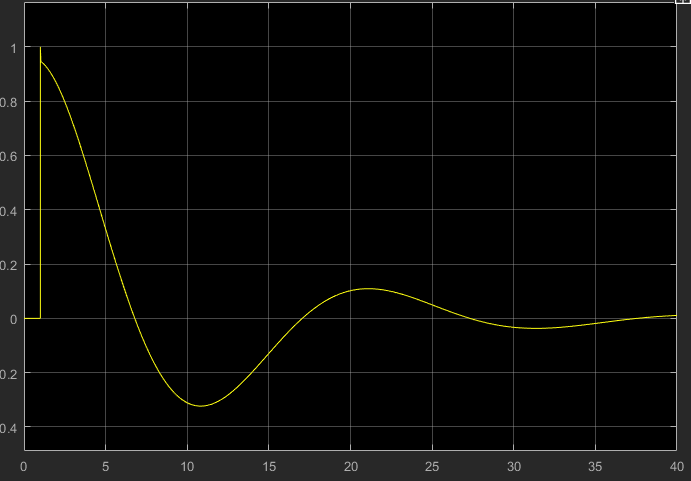
\includegraphics[width=\imagewidth]{images/slope_tracking.png}
    \caption{Tracking behaviour of the system.}
    \label{fig:tracking}
\end{figure}

\clearpage
